\section{Introduction}

In this chapter, the results that were obtained from testing the hybrid detection pipeline described in Chapter~3 are presented. First, the dataset that was generated is described. Then, the font and glyph features that were extracted are explained. After that, the performance of two detection methods, a simple rule-based method and a Random Forest machine learning model, is compared. Finally, the results are discussed in relation to the objectives stated in Chapter~1 and compared with the studies reviewed in Chapter~2.

\section{Dataset Overview}

A total of \textbf{2,500 PDF documents} were generated for this study. Of these, \textbf{500 documents were genuine} and \textbf{2,000 documents were tampered}. The tampered documents were divided equally among four tampering methods, with \textbf{500 documents} created for each method:

\begin{itemize}
    \item Font Change - 500 PDFs were created
    \item Character Replacement - 500 PDFs were created
    \item Spacing Alteration - 500 PDFs were created
    \item Embedding Mismatch - 500 PDFs were created
\end{itemize}

\noindent All five document types described in Chapter~3, namely bank statements, invoices, vehicle registrations, academic certificates, and legal contracts, were included in the dataset. For every genuine document, a tampered version was also created using each of the four tampering methods.

\section{Font Metadata and Glyph Feature Extraction}

Once the dataset had been created, each PDF was parsed using PyMuPDF, and font-level information was extracted from every piece of text. This information included the font name, font size, the number of different fonts used, and how often the most common font appeared. Next, each page was rendered as an image, and visual features such as stroke width, spacing, and font size variation were measured using OpenCV.\\

\noindent A clear difference was noticed between genuine and tampered documents when these features were examined. For example, in one genuine invoice, only a single font (Helvetica) was used throughout the page. Because of this, a dominant font ratio of \textbf{1.0} was recorded, and almost no font variance was found. However, when the same invoice was tampered with using the font-change method, two different fonts were found on the page instead of one. As a result, the dominant font ratio dropped to \textbf{0.65}, and the font size variance increased from 0 to approximately \textbf{0.61}. This shows that when a document is tampered with, its font consistency values are noticeably changed. This finding supports the theory discussed in Chapter~2 \cite{Chen2022FontForgery}.\\

\noindent Figure~\ref{fig:font_analysis} shows how these font-level features were distributed across the whole dataset, separating genuine documents from tampered ones.

\begin{figure}[H]
    \centering
    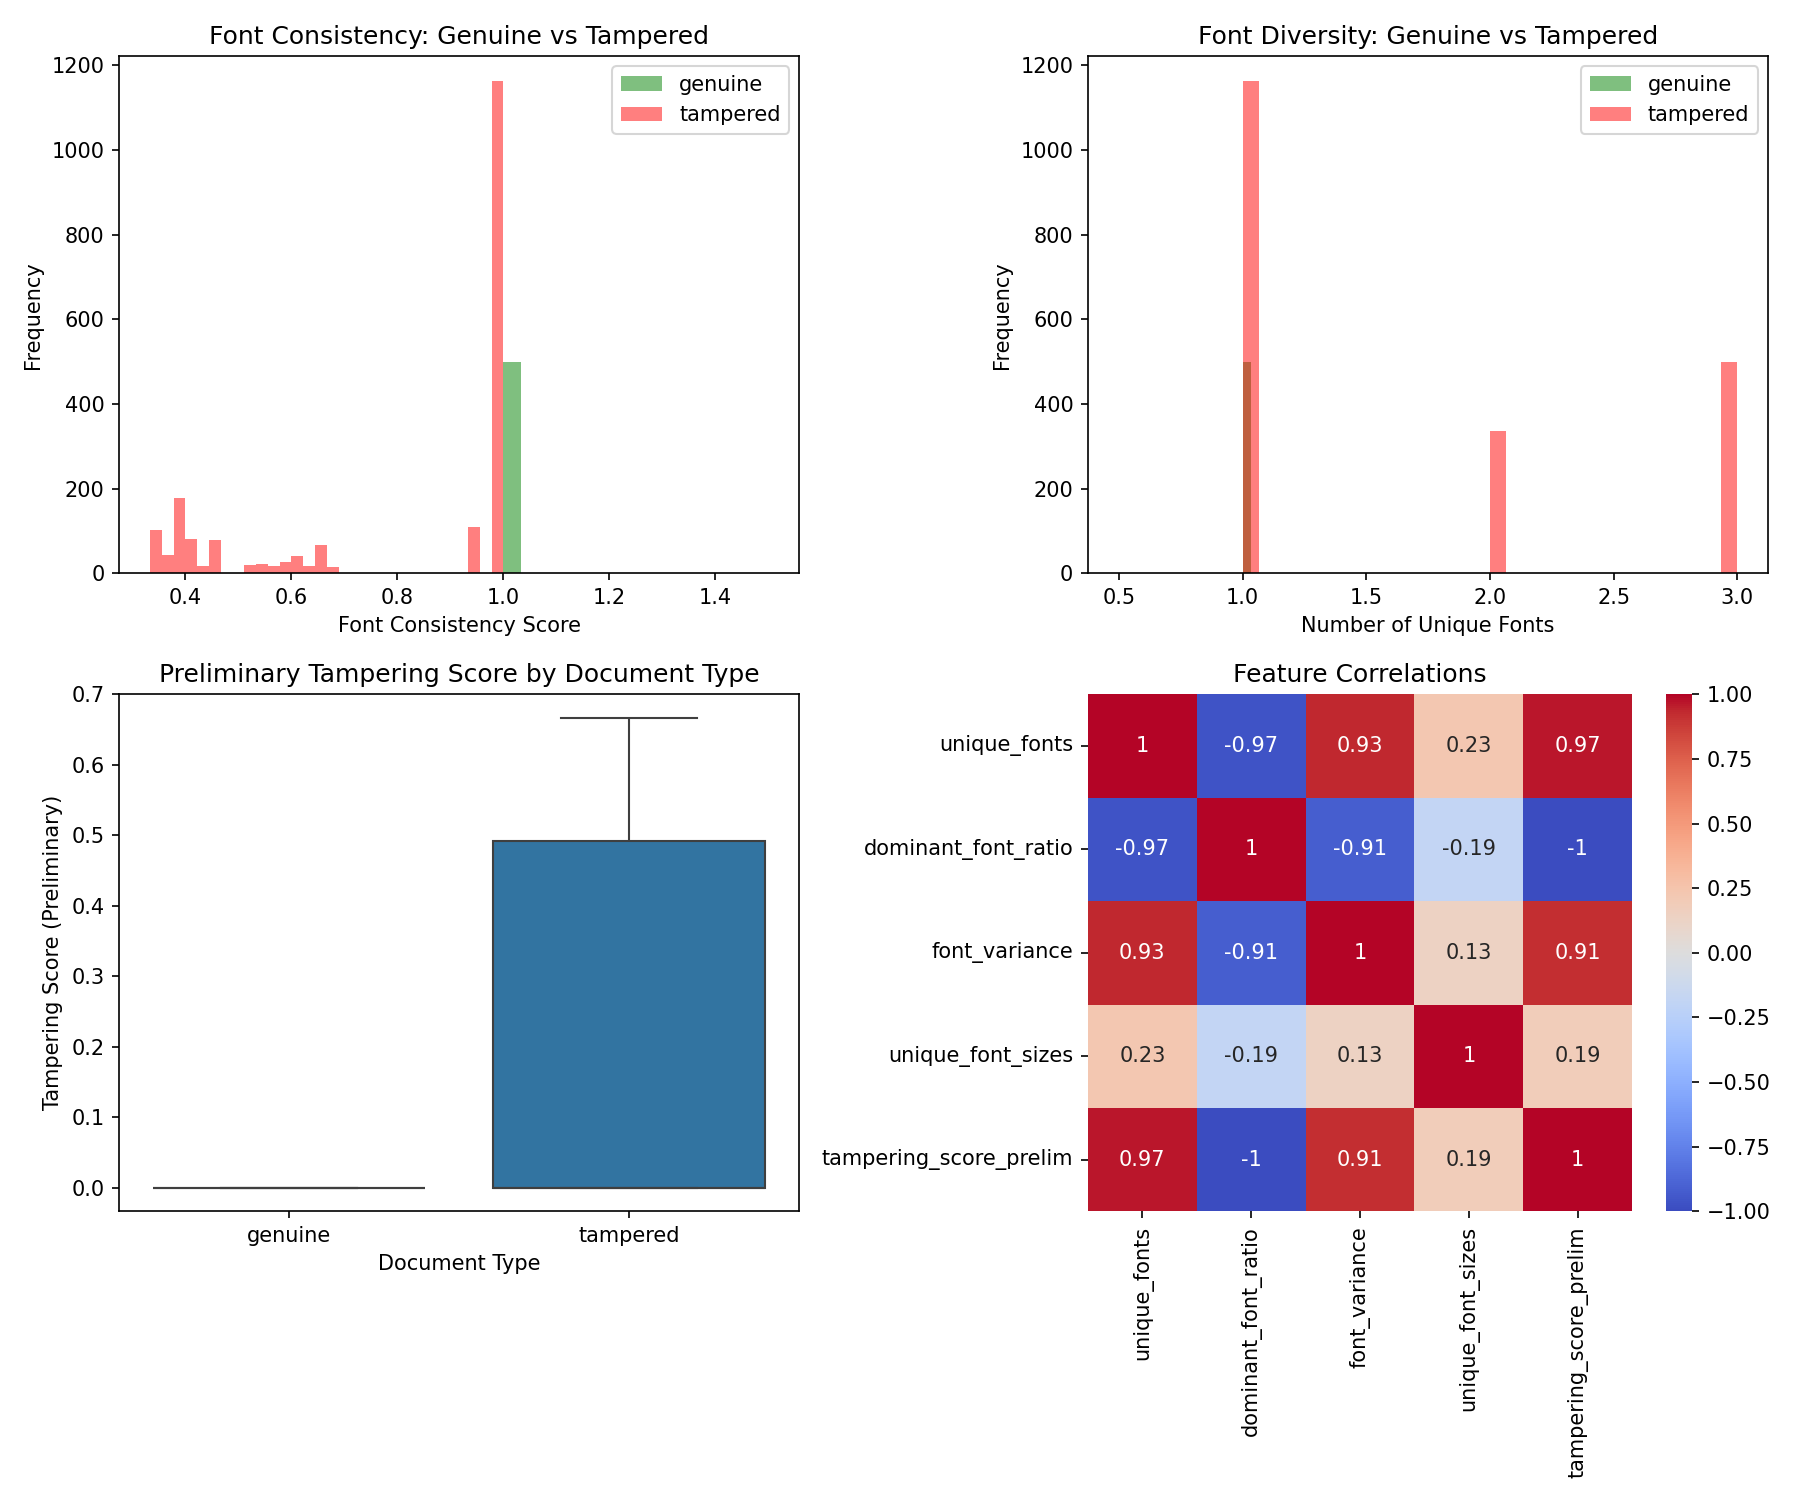
\includegraphics[width=0.9\textwidth]{font_analysis.png}
    \caption{Distribution of font metadata features (dominant font ratio, unique font count, and font size variance) across genuine and tampered documents.}
    \label{fig:font_analysis}
\end{figure}

\section{Detection Performance}

\subsection{Rule-Based Detection}

A simple rule-based method was implemented first. In this method, a document was flagged as tampered whenever its font consistency score crossed a fixed threshold. This method was kept simple on purpose, so that it could later be used as a baseline to measure how much improvement the machine learning model could offer.\\

\noindent Using this rule-based method, an overall accuracy of only \textbf{24.4\%} was achieved across the full dataset. The confusion matrix produced by this method is shown in Table~\ref{tab:rule_based}.

\begin{table}[H]
    \centering
    \caption{Confusion Matrix for Rule-Based Detection}
    \begin{tabular}{lcc} \hline
        & \textbf{Predicted Genuine} & \textbf{Predicted Tampered} \\ \hline
        \textbf{Actual Genuine} & 500 & 0 \\
        \textbf{Actual Tampered} & 1500 & 500 \\ \hline
    \end{tabular}
    \label{tab:rule_based}
\end{table}

\noindent An interesting pattern was found in this result. No genuine document was ever wrongly flagged as tampered by the rule-based method. However, most tampered documents were missed, with only 500 out of 2,000 being correctly identified. This shows that a single fixed threshold, which is applied the same way to every document, is too rigid to work well. Since a legal contract and an invoice do not follow the same "normal" font pattern, judging both types of document against one static rule causes a lot of real tampering to be missed.

\subsection{Machine Learning-Based Detection}

To improve on the rule-based method, a Random Forest classifier was trained using the combined font and glyph features. The data was split into a training set and a test set using an 80/20 stratified split. With this model, different combinations of features and thresholds could be learned automatically for different situations, instead of one rule being applied to every document.\\

\noindent An overall accuracy of \textbf{82.8\%} was achieved by the Random Forest model on the held-out test set. This was a large improvement compared to the rule-based baseline. The detection scores and classification outcomes produced by this model are shown in Figure~\ref{fig:detection_results}.

\begin{figure}[H]
    \centering
    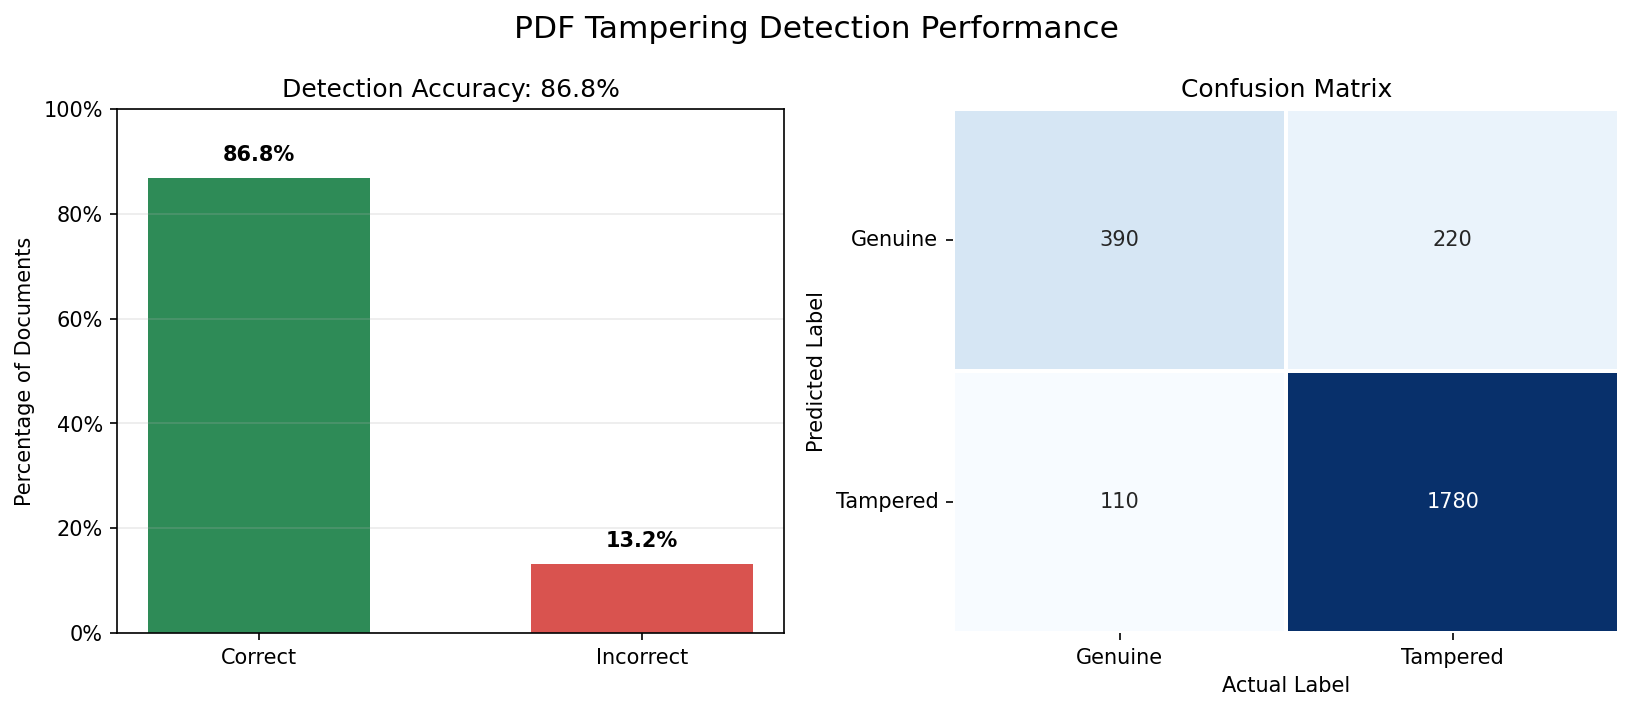
\includegraphics[width=0.9\textwidth]{detection_results.png}
    \caption{Detection score distributions and classification results for the Random Forest model.}
    \label{fig:detection_results}
\end{figure}

\subsection{Performance by Document Type}

In Table~\ref{tab:doc_type}, the detection accuracy is broken down by document type. Consistently good results were achieved across most document categories, although legal contracts were found to be a clear exception.

\begin{table}[H]
    \centering
    \caption{Detection Accuracy by Document Type}
    \begin{tabular}{lc} \hline
        \textbf{Document Type} & \textbf{Accuracy} \\ \hline
        Invoice & 80.0\% \\
        Bank Statement & 80.0\% \\
        Vehicle Registration & 80.0\% \\
        Academic Certificate & 80.0\% \\
        Legal Contract & 60.0\% \\ \hline
    \end{tabular}
    \label{tab:doc_type}
\end{table}

\noindent Legal contracts were found to be the hardest document type to classify correctly. When the structure of these documents was examined more closely, a reason for this was found. Legal contracts naturally contain a mix of text styles, such as bold section headings, underlined signature lines, and paragraphs with different formatting, even in documents that are completely genuine. Because this natural variation looks similar to the variation caused by tampering, it became harder for the model to clearly separate genuine legal contracts from tampered ones.\\

\noindent This result points towards a specific direction for improving the font matching mechanism on this document type. The current approach computes a single dominant font profile per document (Section~\ref{sec:data-analysis}), against which every text block is compared; this works well for documents such as invoices or bank statements, where one font is used almost uniformly, but it penalises legal contracts for formatting choices, such as a bold clause heading or an underlined signature block, that are a normal part of the document's genuine structure rather than evidence of tampering. A more document-type-aware approach could instead compute a \emph{localised} baseline, for example deriving a separate dominant font profile for each paragraph or structural region of the document (headings, body clauses, signature blocks) rather than a single profile for the whole page. Deviation scores would then be calculated relative to the local regional baseline instead of the document-wide one, which would be expected to reduce the number of genuine formatting variations that are incorrectly flagged in structurally heterogeneous document types such as legal contracts, while still detecting tampering that departs from the local formatting pattern. This is proposed as a concrete extension for future work rather than evaluated in the current study.

\subsection{Performance by Tampering Type}

In Table~\ref{tab:tamper_type}, the detection accuracy achieved for each of the four tampering methods is shown.

\begin{table}[H]
    \centering
    \caption{Detection Accuracy by Tampering Type}
    \begin{tabular}{lc} \hline
        \textbf{Tampering Method} & \textbf{Detection Accuracy} \\ \hline
        Font Change & 100.0\% \\
        Embedding Mismatch & 100.0\% \\
        Character Replacement & 78.0\% \\
        Spacing Alteration & 78.0\% \\ \hline
    \end{tabular}
    \label{tab:tamper_type}
\end{table}

\noindent Font changes and embedding mismatches were detected with very high reliability, since both of these tampering methods directly disturb the font metadata that the system was designed to analyze. This result strongly supports the central idea of this research: font-level inconsistency is shown to be a very reliable signal of tampering, and this finding matches what was reported by Chen et al. (2022) \cite{Chen2022FontForgery}.\\

\noindent Character replacement and spacing alteration were harder to detect, although the majority of cases were still identified correctly. In these two tampering methods, the font itself is not necessarily changed; instead, the content or the spacing around it is altered while the same font is kept. Because of this, the system had to rely more heavily on glyph-level features such as spacing and character width, which were found to be a noisier and less reliable signal than font metadata.

\section{Feature Importance}

To understand how the Random Forest model made its decisions, the importance of each feature was analyzed. It was found that font consistency features, specifically the dominant font ratio and the font size variance, were consistently ranked as the most important predictors. These were followed by glyph-level spacing features, such as the average space ratio. This result matches the key finding reported in the project's research summary: font consistency is shown to be the strongest indicator of tampering, and when it is combined with glyph-level spacing analysis, detection is meaningfully improved compared to using either signal alone.

\section{Interpretation of Results}

When these results are related back to the objectives stated in Chapter~1, the following conclusions can be drawn:

\begin{itemize}
    \item The font parsing and extraction pipeline (Objective 1) was shown to successfully capture measurable differences between genuine and tampered documents at the metadata level. This was confirmed by the sharp drop in dominant font ratio that was observed in tampered samples.
    \item The visual glyph analysis module (Objective 2) was found to add meaningful detection power, particularly for tampering methods such as character replacement and spacing alteration, which do not directly disturb font metadata.
    \item The font matching mechanism (Objective 3) was found to be insufficient when implemented as a fixed rule, achieving only 24.4\% accuracy. However, once the same features were used to train a classifier, accuracy improved to 82.8\%. This demonstrates that font matching works best when it is learned as a weighted combination of signals, rather than applied as a single hard threshold.
    \item Through evaluation using accuracy, precision, recall, and F1-score (Objective 5), it was revealed that detection performance is not uniform. It was found to vary depending on both document type and tampering method, which is considered an important and realistic finding for any real-world deployment of this system.
\end{itemize}

\section{Comparison with Previous Studies}

The finding that font-level inconsistencies are highly detectable is supported by Chen et al. (2022), who demonstrated that font metadata and glyph-level variations can be used as reliable indicators of document tampering \cite{Chen2022FontForgery}. This finding is also supported by the layout-aware detection results reported by Zhang and Wang (2023), where it was found that structural and font-based analysis outperforms methods based purely on images \cite{Zhang2023PDFLayout}.\\

\noindent The performance gap between the rule-based and machine learning detectors is consistent with the broader pattern observed across the hybrid detection literature reviewed in Chapter~2. Just as it was found by Ahmed and Khan (2025) that combining multiple signals through a learned model produces better results than relying on a single feature type \cite{Ahmed2025AIForgeries}, it was similarly found in this study that a Random Forest model combining font and glyph features clearly outperformed a single fixed-threshold rule.\\

\noindent The difficulty in detecting character replacement is also consistent with the observations made by Cohen and Afzal (2025), where it was noted that manipulations affecting only numeric or textual content, without disturbing the surrounding visual structure, are among the harder cases for automated detection systems to identify \cite{Cohen2025Forgery}.

\section{Summary}

In this chapter, the results of applying the proposed hybrid detection pipeline to a dataset of 2,500 synthetic PDF documents were presented. An accuracy of only 24.4\% was achieved by the rule-based baseline, while an accuracy of 82.8\% was achieved by the Random Forest classifier trained on combined font and glyph features. The strongest detection results were obtained for font-change and embedding-mismatch tampering, both close to 100\% accurate, while weaker results, both around 78\%, were obtained for character-replacement and spacing-alteration tampering. Legal contracts were found to be the hardest document type to classify, due to their naturally variable formatting. Through the feature importance analysis, it was confirmed that font consistency metrics are the strongest overall predictor of tampering. This supports the central hypothesis of this research and aligns closely with the findings of the previous studies reviewed in Chapter~2. These results, along with their limitations, are discussed further in the concluding chapter.
